\chapter{Нелинейные колебания оболочек}\label{ch:ch3}

\section{Обзор} \label{ch:ch3/sec1}

{\color{blue}
В данной вводной части будет уделен акцент в основном пластинам и оболчкам из ФГМ, и немного затронуты оболочки из композиционного материала, но можно распространить и на други виды конструкций и материалов.


Произведем беглый обзор литературы посвященой геометрически нелинейным свободным и вынужденным колебаниям оболочек из традиционных и современных материалов. Плоские и несовершенные пластины и мембраны исключены из рассмотрения. В общем виде рассматриваются замкнутые оболочки и изогнутые панели из функционально-градиентных и композитным материалов; внимание уделяется нелинейным колебаниям оболочек. Теоретические, численные и экспериментальные исследования посвященные конкретным динамическим проблемам, включающим параметрические колебаний, устойчивости, динамического смятия, нестационарных колебаний и хаотические колебания.
}

Оболочечные конструкции используются в самолетах, космических аппаратах, ракетах, автомобилях, компьютерах, подводных лодках, катерах, резервуарах для хранения и даже крышах зданий.

В последнее десятилетие непрерывное развитие материаловедения и инженерии, наряду с растущим спросом на производство легких конструкций, привело к использованию передовых материалов (слоистых композитов и функционально-градиентных материалов (ФГМ)) при проектировании оболочечных конструкций. Среди разнообразных областей применения, аэрокосмическая и авиационная области являются особенно сложными, так как они включают в себя взаимодействие жидкостей  и конструкции и использование новых материалов с мало-известными свойствами. Для этого необходимо разрабатывать модели, учитывающие нелинейные эффекты, такие как большие деформации, а также уметь предсказывать реакцию конструкции на большие амплитудные колебания.


В случае линейных колебаний замкнутых (по окружности) цилиндрических оболочек, подверженных радиальным периодическим возбуждениям, форма моды оболочки представляет собой стоячую волну, непосредственно возбуждаемую внешним возбуждением, которая представляет собой число \(n\) узловых диаметров. Такая мода называется вынужденной. При колебаниях оболочек с большой амплитудой существует внутренний резонанс один к одному между \textbf{управляемой} модой и ортогональной модой, имеющей ту же форму и собственную частоту, что и управляемая мода, но повернутой на \(\pi/2n\), известной как \textbf{сопутствующая} мода. 

Такое взаимодействие мод приводит к появлению отклика бегущей волны в окружном направлении оболочки, который проявляется даже при амплитудах колебаний, меньших, чем толщина оболочки. Фактически, наличие отклика бегущей волны вблизи резонанса имеет принципиальное отличие от линейных колебаний. 


Другой важной особенностью замкнутых круговых цилиндрических оболочек при колебаниях большой амплитуды является динамическое осесимметричное сжатие, которое было рассмотрено как теоретически, так и экспериментально. В частности, при колебаниях большой амплитуды оболочка испытывает внутреннее осесимметричное динамическое сжатие с удвоенной частотой возбуждения, что гарантирует квазинерастяжимость оболочки в плоскости. Без этого осесимметричного сжатия оболочка значительно увеличила бы свою длину по окружности, что противоречит механике оболочек. На самом деле, оболочки легче изгибаются, чем растягиваются.

Оболочки подверженные нагрузкам в плоскости, теряют устойчивость и разрушаются после определенного порога. Фактически, при наличии статических нагрузок в плоскости неустойчивость возникает через вилообразную бифуркацию (Pitchfork bifurcation), в то время как при периодических нагрузках в плоскости так называемая параметрическая неустойчивость возникает через бифуркацию удвоения периода в соседней области частот, вдвое превышающей собственные частоты изгибной моды. В последнем случае, в отличие от нелинейных колебаний оболочек из-за радиального гармонического возбуждения, неустойчивость может возникнуть даже при малых амплитудах возбуждения и намного ниже статической нагрузки смятия.


Оболочки, заполненные жидкостью, имеют более низкие собственные частоты вследствие дополнительной виртуальной массы самой жидкости. В цилиндрических оболочках эффект добавленной виртуальной массы ниже для асимметричных мод, чем для осесимметричных мод. Поэтому нелинейность, проявляемая тонкими замкнутыми круговыми оболочками, усиливается присутствием вязкой жидкости. Более того, круговые цилиндрические оболочки, поддерживаемые или зажатые с обоих концов и транспортирующие жидкость, теряют устойчивость через дивергенцию, которая представляет собой статическую вилообразную бифуркацию равновесия, когда скорость потока  достигает критического значения. Дивергенция является сильно субкритической, становясь сверхкритической для высоких скоростей потока flow.  В этом случае система имеет два или более устойчивых решений, связанных с дивергенцией, намного раньше, чем возникает вилочная бифуркация. Другими словами, если оболочка возмущена от начальной конфигурации, она может иметь сильные деформации, приводящие к разрушению намного ниже критической скорости, которая может быть предсказана линейным анализом.

В отличие от замкнутых круговых цилиндрических оболочек, криволинейные панели (т.е. открытые оболочки, с одинарной и двойной кривизной) не всегда демонстрируют внутренний резонанс, если только для определенных соотношений толщины и площади, и не имеют осесимметричного динамического сжатия.  Особенности панелей, которые делают нелинейный анализ этих структур интересным, - это асимметричный характер колебаний относительно исходной недеформированной средней поверхности, нелинейное поведение смягчения, переходящее в упрочнение при колебаниях большой амплитуды, и различные условия внутреннего резонанса, которые могут иметь место для различных форм.


\subsection{Краткий обзор нелинейных теории оболочек} \label{ch:ch3/sec1/sub1}

Классические теории нелинейной механики оболочек, подходящие для тонких оболочек, включают теории Доннелла \cite{donnel1934}, Новожилова \cite{novozhilov1953}, Сандерса \cite{sanders1963}, Койтера \cite{koiter1966} и Флюгге Лурье Бирна \cite{ginsberg1973}, которые все основаны на гипотезах Кирхгофа-Лява. В частности, нелинейная теория мелких оболочек Доннелла пренебрегает инерцией в плоскости и дает точные результаты только для очень тонких оболочек. В этой теории смещения в плоскости являются бесконечно малыми, в то время как поперечные смещения порядка толщины оболочки. Более того, нелинейные члены сохраняются только в поперечном сдвиге (нелинейные члены типа фон Кармана, по аналогии с рассмотрением пластин); однако другие эффекты, такие как нелинейность, связанная с плоскими смещениями, игнорируются. Теория Доннелла, без гипотезы тонкой оболочки, сохраняет инерцию в плоскости и является более точной, чем нелинейная теория тонкой оболочки Доннелла; однако, она сохраняет нелинейные члены только типа фон Кармана. Теория Сандерса - это более расширенная нелинейная теория оболочек, разработанная Сандерсом \cite{sanders1963} первоначально в тензорной форме. Эта же теория была получена независимо Койтером \cite{koiter1966} примерно в тот же период, что привело к обозначению этой теории как нелинейной теории оболочек Сандерса-Койтера. Эта теория подходит для конечных перемещений с малыми деформациями и умеренно малыми вращениями. Поэтому в теории Сандерса-Койтера смещения в плоскости не являются бесконечно малыми, а в соотношениях деформационных смещений существуют нелинейные члены, которые зависят как от смещений в плоскости, так и от поперечных смещений. В теориях Доннелла и Сандерса-Койтера изменения кривизны и кручения средней поверхности предполагаются линейными. Более того, теория Сандерса-Койтера дает точные результаты для амплитуд колебаний, значительно превышающих толщину оболочки, в то время как теория Доннелла точна только для очень тонких оболочек и мод с высоким окружным числом волн.


Общие нелинейные теории оболочек, разработанные Новожиловым \cite{novozhilov1953}, и теория Флюгге-Лур'е-Бирна \cite{ginsberg1973} очень похожи и отличаются только в плане замены кривизны и кручения. В обеих теориях можно сохранить нелинейность в изменениях кривизны и кручения \cite{amabili2008}. Более того, предположение о тонкости сохраняется в выводах обеих теорий, а соотношения деформационных сдвигов включают нелинейности как в поперечных, так и в плоских перемещениях. Все эти классические теории получены путем пренебрежения деформацией поперечного сдвига и инерцией вращения, и поэтому могут давать неточные результаты для умеренно толстых или слоистых анизотропных оболочек. Для того чтобы преодолеть это ограничение, были введены теории сдвиговой деформации. Эти теории можно разделить на теории деформации сдвига первого порядка и теории деформации сдвига более высокого порядка; в первой категории для равновесия требуется поправочный коэффициент сдвига, поскольку предполагается равномерная деформация сдвига по толщине оболочки. Теории деформации сдвига более высокого порядка преодолевают это ограничение, поскольку предполагается реалистичное распределение напряжения сдвига по толщине оболочки, что также удовлетворяет условию нулевого напряжения сдвига на верхней и нижней поверхностях оболочки. Эти теории были полностью рассмотрены в книгах Амабили \cite{amabili2008}, Редди \cite{reddy2004} и Каррера и др \cite{carreranali2011}. Более того, теории линейной сдвиговой деформации и зигзагообразной деформации (слои с постоянным углом сдвига) были подробно рассмотрены Каррерой \cite{carrera2002, carrera2003},  и Редди и Арсиньегой \cite{reddyarciniega2004}.


Нелинейная теория деформации сдвига первого порядка была впервые предложена Редди и Чандрашекхарой [18] и основана на нелинейных членах Сандерса-Койтера. Для описания деформаций оболочки использовались пять независимых переменных: три перемещения и два вращения. Нелинейная теория сдвиговых деформаций оболочек первого порядка, основанная на нелинейных членах типа фон Кармана, и ее формулировки в виде отдельных элементов также приведены в работе Редди [13]. Либреску [19] разработал нелинейную теорию оболочек, расширив смещения оболочки кубическими членами в поперечной координате. Деннис и Палазотто [20] и Палазотто и Деннис [21] расширили линейную теорию оболочек Редди высшего порядка со сдвиговой деформацией до нелинейной деформации, введя нелинейные члены типа фон Кармана. Нелинейная теория оболочек высшего порядка для многослойных анизотропных оболочек с поперечно сжимаемым ядром была разработана Хохе и Либреску [22]. В их теории гипотезы Кирхгофа-Лява были приняты для торцевых поверхностей, а для перемещений ядра рассматривалось разложение в ряд мощности второго/третьего порядка. Чаудхури [23] разработал теорию нелинейного зигзага для нелинейного конечно-элементного анализа двояковыпуклых оболочек путем рассмотрения полных нелинейных соотношений деформационных перемещений для пяти независимых переменных оболочки. Амабили и Редди [24] разработали новую теорию для закрытых и открытых оболочек, которая, в отличие от предыдущих нелинейных теорий оболочек, была выведена с сохранением инерции вращения, деформации сдвига и нелинейности в плоскости и поперечных смещениях. Новая теория показала превосходство над существующими нелинейными теориями деформации сдвига при прогнозировании колебаний большой амплитуды глубоких и умеренно толстых ламинированных круговых цилиндрических оболочек [25] и изогнутых панелей [26]. Недавно Амабили [27] расширил теорию [24], добавив эффект растяжения толщины и приняв во внимание геометрические несовершенства. В этой новой теории для описания деформации оболочки использовались шесть независимых переменных. В частности, в [27] предполагается равномерная поперечная нормальная деформация по всей толщине оболочки. Эта теория была расширена до поперечной нормальной деформации третьего порядка Амабили [28]. Преимущества теорий оболочек, сохраняющих поперечные нормальные напряжения и деформации, заключаются в использовании полных трехмерных определяющих уравнений, и они особенно подходят для мягких материалов, таких как резины и биологические материалы, где достигаются очень большие деформации, сопровождающиеся большим уменьшением толщины. Parisch [29] и Sansour [30] разработали независимые теории оболочек, которые вводят квадратичное предположение о смещении оболочки по толщине оболочки. Более того, точная линейная теория оболочек, учитывающая изменение толщины, была разработана Каррерой и другими [31] и Феррейрой и другими [32]. Геометрически нелинейные теории оболочек на тензорной основе достаточно широко представлены в литературе [33 45]. Еремеев и Петрашкевич [33] разработали общую нелинейную теорию оболочек с учетом фазовых переходов материалов. В их теории смещения оболочек выражались через усредненные по работе переводы и повороты поперечных сечений оболочек. Более того, все связи оболочек были найдены из вариационного принципа стационарной потенциальной энергии. Опока и Петрашкевич [34] последовательно получили полную краевую задачу для нелинейной теории тонких упругих оболочек, выраженную в терминах результирующих напряжений и изгиба опорной поверхности оболочки. Арсиньега и Редди [35] разработали усовершенствованную теорию деформации сдвига первого порядка с семью независимыми переменными в рамках метода Лагранжа и представили формулы конечных элементов, которые могут быть использованы для изучения нелинейного анализа широкого спектра геометрий оболочек из различных типов материалов, включая изотропные, слоистые композиты и МГП. Опока и Петрашкевич [36] модифицировали свою предыдущую работу [34], сформулировав новую версию лагранжевой теории тонких оболочек в терминах смещений опорной поверхности и на основе принципа виртуальной работы. Бердичевский [37] предложил нелинейную теорию для многослойных оболочек, основанную на асимптотическом вариационном методе. Шен и др. [38] разработали модифицированную теорию оболочек Койтера и обсудили роль метрических тензоров и тензоров кривизны в построении нелинейных моделей упругих оболочек типа Койтера. Петрашкевич [39] рассмотрел некоторые эквивалентные выражения тензора изгиба в нелинейной теории оболочек и указал, что выражение, предложенное Шеном и другими [38], не является точным. Теория оболочек Койтера также обсуждалась с точки зрения нелинейной трехмерной упругости Штайгманом [40]. Нелинейные теории оболочек, которые были предложены с использованием континуума Коссерата, можно найти в работах. [41 45]. 


Основной идеей этого варианта модели механики сплошной среды является независимость перемещений и вращений, а значит, по аналогии, независимость сил и моментов. Нелинейная теория микрополярных оболочек была дана в работе [41], а локальная группа симметрии для модели континуальной механики - в работе [41], а локальная группа симметрии для динамической точной теории оболочек установлена в работе [42]. Краткий обзор теорий Коссерата для оболочечных структур был проведен Альтенбахом и другими [44], а нелинейная теория оболочек в наномасштабе была представлена Альтенбахом и Ермеевым [45]. Более того, нелинейная теория градиента деформации оболочек была представлена Лазопулосом и Лазопулосом [46].


{\color{blue} не дошел до ФГМ материалов}


\section{Свободные колебания объединенных цилиндрическо-полусферических оболочек из ФГМ} \label{ch:ch3/sec2}

\subsection{Введение} \label{ch:ch3/sec2/sub1}

В данном обзоре анализируется реакция свободных колебаний системы соединенных оболочек, включающей цилиндрическую и сферическую оболочки. Предполагается, что система соединенных оболочек изготовлена из функционально-градиентного материала (ФГМ). Предполагается, что свойства оболочек градируются по толщине. Обе оболочки имеют одинаковую толщину. Для учета эффектов сдвиговых деформаций по толщине и вращательной инерции используется теория сдвиговых деформаций оболочек первого порядка. Для создания общих уравнений движения и соответствующих граничных условий и условий неразрывности с помощью принципа Гамильтона принимаются кинематические предположения типа Доннелла. Полученная система уравнений дискретизируется с помощью полуаналитического метода обобщенных дифференциальных квадратур. Учитывая зажатые и свободные граничные условия для торца цилиндрической оболочки и условия непрерывности пересечения, ставится задача на собственные значения для исследования частот вибрации соединенной оболочки. После доказательства эффективности и обоснованности настоящего метода для случая тонких изотропных однородных соединенных оболочек, проводятся некоторые параметрические исследования для системы объединенных цилиндрических сферических оболочек умеренной толщины. Новые результаты представлены для случая соединенных оболочек ФГМ, чтобы исследовать влияние степенной функции при задании свойств.


Вибрации сложных оболочек привлекают внимание в последние годы [1-3*]. Система соединенных цилиндрических и сферических оболочек широко используется во многих промышленных приложениях, таких как сосуды под давлением и архитектурные сооружения. Для этих конструкций известно, что вблизи соединенного участка возникают локализованные и сильные изгибающие моменты, когда оболочка подвергается внезапным нагрузкам. Вибрации, вызванные такими нагрузками, могут привести к явлению усталости. Поэтому понимание вибрационных свойств соединенных оболочек представляет большой интерес и важность для установления основных требований к безопасной конструкции.


Вибрация соединенных сферо-цилиндрических оболочек или цилиндрических оболочек с различным креплением концов была темой иссследования. Например, собственные частоты цилиндрических оболочек, зажатых с одного конца и закрытых с другого конца различными типами оболочек вращения (конусы, полусферы, эллипсоиды и т.д.), изучены Галлетли [16*]. Ли и др. [17*] провели исследование свободных колебаний комбинированных цилиндрических и сферических оболочек. В этом исследовании рассматриваются различные случаи граничных условий. Для решения задач на собственные значения, связанных с собственными частотами и формами мод системы тонких оболочек Флюгге, разработаны решения на основе метода Рэлея-Ритца. Показано, что колебательное поведение объединенной сферо-цилиндрической оболочечной структуры не зависит от мелкости полусферической оболочки, в то время как длина цилиндрической оболочки влияет на колебательное поведение объединенной полусферо-цилиндрической оболочки. Ву и др. [18*], используя теорию оболочек Рейсснера-Нагди-Берри, применили метод разложения доменов (DDM) для исследования вибрационных характеристик объединенной цилиндрическо-сферической оболочки с различными граничными условиями. В другом исследовании Ву и др. [19*] сосредоточились на свободных колебаниях объединенной цилиндрическо-сферической оболочки с упругими опорными типами граничных условий, используя метод разложения доменов. Используя теорию оболочек Флюгге и энергетический метод Рэлея-Ритца, Йосефзад и другие [20*] проанализировали характеристики свободных колебаний предварительно напряженных соединенных сферо-цилиндрических оболочек со свободными граничными условиями. В модальном испытании для расчета форм мод и собственных частот объединенной оболочечной конструкции используется программное обеспечение LMS. Ку и др. [21*] проанализировали свободные колебания системы соединенных цилиндро-конических оболочек с классическими или неклассическими граничными условиями. В качестве фундаментальных теоретических предположений используются предположения теории Рейсснера-Нагди о тонкой оболочке. Непрерывность границы раздела и геометрические граничные условия приблизительно выполняются с помощью модифицированного вариационного принципа и метода взвешенных остатков наименьших квадратов. Ку и его соавторы также применили свой предыдущий метод [21*] для анализа свободных колебаний кольцевых жестко соединенных коническо-цилиндрических оболочек [22*], соединенных коническо-цилиндрических сферических оболочек [23*], соединенных цилиндрическо-сферических оболочек с упругими граничными условиями [24*] и сферическо-цилиндрических сферических оболочек [25*]. В серии работ Канг[26-28*] исследовал отклик свободных колебаний цилиндрических оболочек, закрытых различными типами оболочек вращения в рамках трехмерной теории упругости. Были определены полная деформация и кинетическая энергия объединенной системы оболочек, а метод Ритца с классическими полиномиальными функциями использовался для решения задачи собственных значений и выделения собственных частот.


Существует лишь несколько работ, посвященных свободным колебаниям соединенных цилиндрических сферических оболочек, причем большинство из них ограничивается классом тонких оболочек. Кроме того, все исследования касаются однородного класса оболочек, а о свободных колебаниях цилиндрических сферических оболочек, соединенных FGM, пока не сообщается. Целью настоящего исследования является изучение характеристик свободных колебаний объединенной цилиндрическо-сферической оболочечной структуры, изготовленной из ФГМ, с использованием модели сдвиговой деформируемой оболочки первого порядка, подходящей для оболочек умеренной толщины. Кинематические допущения типа Доннелла используются для установления уравнений движения и соответствующих граничных условий. Для дискретизации уравнений движения разработана полуаналитическая процедура, основанная на разложении Фурье вдоль окружного направления и дискретизации GDQ вдоль тангенциального направления. Метод GDQ также применяется к непрерывности пересечения и граничным условиям. Создана система однородных задач с собственными значениями, которая может быть полезна для исследования частот объединенных цилиндрическо-сферических оболочек. После проверки предложенного метода решения с помощью некоторых сравнительных исследований, проводится серия параметрических исследований для изучения влияния индекса силового закона, длины цилиндрической оболочки и радиуса оболочки.

\begin{figure}[h!]
	\centering
	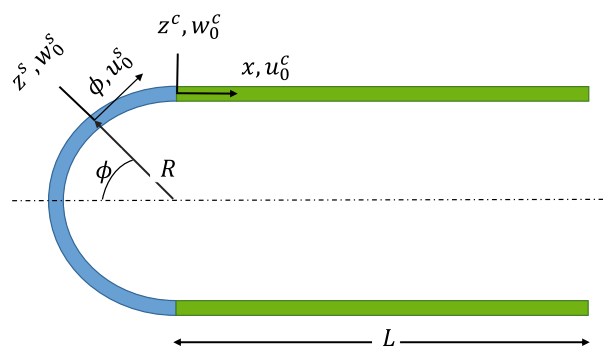
\includegraphics[width=0.75\textwidth]{vibro1_figure1.png}%
	\caption{Геометрические параметры и заданные системы координат объединенной цилиндрической и сферической оболочки}
	\label{fig:vibro1:1}
\end{figure}

\subsection{Описание свойств ФГМ} \label{ch:ch3/sec2/sub2}
Предполагается, что свойства материала керамической и металлической составляющих системы соединенных оболочек распределены по толщине на основе степенной функции. Предполагается, что объемная доля керамики \(V_c\) и объемная доля металла \(V_m\) подчиняются следующей форме [29-36*].

\begin{equation}
	\label{eq:vibro1:1}
	V_c = \left (\frac{1}{2}+\frac{z}{h} \right )^{k} ,\quad  V_m =1 - V_c
\end{equation}


В приведенном выше уравнении \(k\) является показателем функции и диктует распределение свойств материала по толщине. Очевидно, что поверхность \(z = +h/2\) богата керамикой, а поверхность \(z = -h/2\) богата металлом.


Следуя простому правилу подхода смесей (правило Фойгта), каждое свойство объединенной оболочки FG, например P, может быть записано как функция соответствующих свойств составляющих и объемной доли составляющих как

\begin{equation}
	\label{eq:vibro1:2}
	P(z) = P_m + P_{cm} \left (\frac{1}{2}+\frac{z}{h} \right )^{k} ,\quad  P_{cm} = P_c - P_m
\end{equation}

где \(P_m\) и \(P_c\) -- соответствующие свойства металлических и3 керамических компонентов, соответственно. В настоящей работе предполагается, что модуль упругости E и плотность массы \(\rho \) описываются уравнением (\cref{eq:vibro1:2}), а коэффициент Пуассона \(\mu \) считается постоянным по всей толщине, поскольку он изменяется только в небольшом диапазоне.


\subsection{Постановка задачи}\label{ch:ch3/sec2/sub3}

Рассмотрим объединенную цилиндрическо-полусферическую оболочку из функционально-градиентного материала равномерной толщины \(h\), радиуса сферы \(r^s = R\), радиуса цилиндра \(r^c = R\) и длины цилиндра \(L^c = L\). Система показана на \cref{fig:vibro1:1}. Система координат \((x, \theta, z)\) применяется к системе цилиндрической оболочки, а система \((\phi, \theta, z)\) -- к сферической оболочке. Системы координат также показаны на \cref{fig:vibro1:1}.

Чтобы учесть деформации сдвига по толщине и эффекты вращательной инерции цилиндрических и сферических оболочек, для формулировки определяющих уравнений оболочки используется теория сдвиговых деформаций первого порядка (\textbf{FSDT}) оболочек. На основе FSDT компоненты смещения в общей точке для цилиндрических и сферических оболочек могут быть представлены в соответствии с характеристиками средней поверхности таким образом, что

\begin{equation}
	\label{eq:vibro1:3}
	\begin{split}
	u^i (\xi, \theta, z, t) &= u_0^i(\xi, \theta, t)+ z \varphi_{\xi}^i (\xi, \theta,  t)\\
	v^i (\xi, \theta, z, t) &= v_0^i(\xi, \theta, t)+ z \varphi_{\theta}^i (\xi, \theta,  t)\\
	w^i (\xi, \theta, z, t) &= w_0^i (\xi, \theta, t)
	\end{split}
\end{equation}

В приведенном выше уравнении \(u, v, w\) -- это тангенциальное, окружное и поперечное перемещения по толщине, соответственно. Надстрочный индекс \(i\) может быть \(c\) или \(s\) для цилиндрических и сферических оболочек. Кроме того, \(\xi\) может принимать значение \(\phi\) или \(x\) для сферических и цилиндрических оболочек, соответственно. Подстрочный индекс 0 указывает на характеристики срединной поверхности. Кроме того, \(\phi_{\xi}\) и \(\phi_{\theta}\)  -- это, соответственно, повороты поперечных нормалей вокруг осей \(\theta\) и \(\xi\), соответственно.

Согласно FSDT, компоненты поля деформации в произвольной точке цилиндрической или сферической оболочки могут быть получены в терминах срединной поверхности оболочки и изменению кривизны.  Следовательно, можно записать [37*]

\begin{equation}
	\label{eq:vibro1:4}
	\begin{Bmatrix}
		\varepsilon_{\xi \xi}^i \\
		\varepsilon_{\theta \theta}^i \\
		\gamma_{\xi \theta}^i \\
		\gamma_{\xi z}^i \\
		\gamma_{\theta z}^i
	\end{Bmatrix} =
	\begin{Bmatrix}
		\varepsilon_{\xi \xi 0}^i \\
		\varepsilon_{\theta \theta 0}^i \\
		\gamma_{\xi \theta 0}^i \\
		\gamma_{\xi z 0}^i \\
		\gamma_{\theta z 0}^i
	\end{Bmatrix}
	+ z
		\begin{Bmatrix}
			\kappa_{\xi \xi}^i \\
			\kappa_{\theta \theta}^i \\
			\kappa_{\xi \theta}^i \\
			\kappa_{\xi z}^i \\
			\kappa_{\theta z}^i
	\end{Bmatrix}
\end{equation}

где компоненты деформации, связанные со средней поверхностью цилиндрической оболочки, имеют вид

\begin{equation}
\label{eq:vibro1:5}
\begin{Bmatrix}
		\varepsilon_{\xi \xi 0}^{c} \\
		\varepsilon_{\theta \theta 0}^{c} \\
		\gamma_{\xi \theta 0}^{c} \\
		\gamma_{\xi z 0}^{c} \\
		\gamma_{\theta z 0}^{c}
\end{Bmatrix} =
\begin{Bmatrix}
		u_{0, x}^c \\
		\frac{v_{0, \theta}^c}{r^c}+\frac{w_{0}^c}{r^c} \\
		\frac{u_{0, \theta}^c}{r^c}+v_{0, x}^c \\
		w_{0,x}^c+\varphi_{x}^c \\
		\frac{w_{0,\theta}^c}{r^c}-\frac{v_{0}^c}{r^c} + \varphi_{\theta}^c
\end{Bmatrix}
\end{equation}


и аналогично для сферической оболочки получаем

\begin{equation}
	\label{eq:vibro1:6}
	\begin{Bmatrix}
		\varepsilon_{\phi \phi 0}^{s} \\
		\varepsilon_{\theta \theta 0}^{s} \\
		\gamma_{\phi \theta 0}^{s} \\
		\gamma_{\phi z 0}^{s} \\
		\gamma_{\theta z 0}^{s}
	\end{Bmatrix} =
	\begin{Bmatrix}
		\frac{u_{0, \phi}^s}{r^s}+\frac{w_{0}^s}{r^s} \\
		\frac{v_{0, \theta}^s}{r^s \sin{\phi}}+\frac{u_{0}^s}{r^s} \cot{\phi}+\frac{w_0^s}{r^s} \\
		\frac{v_{0, \phi}^s}{r^s} +\frac{u_{0}^s}{r^s \sin{\phi}} -\frac{v_0^s}{r^s}\cot{\phi}\\
		\frac{w_{0, \phi}^s}{r^s} +\varphi_{\phi}^s -\frac{u_0^s}{r^s} \\
		\frac{w_{0,\theta}^c}{r^c}-\frac{v_{0}^c}{r^c} + \varphi_{\theta}^c
	\end{Bmatrix}
\end{equation}

Компоненты изменения кривизны в смысле Доннелла, совместимые с FSDT для цилиндрической оболочки [37*]

\begin{equation}
	\label{eq:vibro1:7}
	\begin{Bmatrix}
		\kappa_{xx}^{c} \\
		\kappa_{\theta \theta}^{c} \\
		\kappa_{x \theta}^{c} \\
		\kappa_{x z}^{c} \\
		\kappa_{\theta z}^{c}
	\end{Bmatrix} =
	\begin{Bmatrix}
		\varphi_{x,x}^c \\
		\frac{\varphi_{\theta, \theta}^c}{r^c} \\
		\frac{\varphi_{x, \theta}^c}{r^c}+\varphi_{\theta, x}^c \\
		0 \\
		0
	\end{Bmatrix}
\end{equation}

а для сферической оболочки могут быть записаны в виде

\begin{equation}
	\label{eq:vibro1:8}
	\begin{Bmatrix}
		\kappa_{\phi\phi}^{s} \\
		\kappa_{\theta \theta}^{s} \\
		\kappa_{\phi \theta}^{s} \\
		\kappa_{\phi z}^{s} \\
		\kappa_{\theta z}^{s}
	\end{Bmatrix} =
	\begin{pmatrix}
		\frac{\varphi_{\phi,\phi}^s}{r^s} \\
		\frac{\varphi_{\theta, \theta}^s}{r^s \sin{\phi}} + \frac{\varphi_{\theta}^s}{r^s}\cot{\phi} \\
		\frac{\varphi_{\theta, \phi}^s}{r^s}+\frac{\varphi_{\phi, \theta}^s}{r^s \sin{\phi}}-\frac{1}{r^s}\varphi_{\theta}^s \cot{\phi} \\
		0 \\
		0
	\end{pmatrix}
\end{equation}


Для случая, когда свойства материала оболочки линейно упругие, компоненты напряжения в виде деформаций рассчитываются как 

\begin{equation}
	\label{eq:vibro1:9}
	\begin{Bmatrix}
		\sigma_{\xi \xi}^i \\
		\sigma_{\theta \theta}^i \\
		\tau_{\xi \theta}^i \\
		\tau_{\xi z}^i \\
		\tau_{\theta z}^i
	\end{Bmatrix} =
	\begin{bmatrix}
		Q_{11} & Q_{12} & 0       & 0  	  & 0 \\
		Q_{12} & Q_{22} & 0       & 0     & 0 \\
		 0     &     0  & Q_{44}  & 0 	  & 0 \\
		 0     &     0  & 0       & Q_{55}& 0 \\
		 0     &     0  & 0       & 0     &  Q_{66}
	\end{bmatrix}
	\begin{Bmatrix}
		\varepsilon_{\xi \xi}^i \\
		\varepsilon_{\theta \theta}^i \\
		\gamma_{\xi \theta}^i \\
		\gamma_{\xi z}^i \\
		\gamma_{\theta z}^i
	\end{Bmatrix}
\end{equation}

где \(Q_{ij}, i,j =1, 2, 4, 5, 6\) являются приведенными коэффициентами жесткости материала и получаются следующим образом

\begin{equation}
	\label{eq:vibro1:10}
	Q_{11} = Q_{22} = \frac{E(z)}{1-\nu^2}, \quad Q_{12}=\frac{\nu E(z)}{1-\nu^2}, \quad Q_{44}=Q_{55}=Q_{66}=\frac{E(z)}{2(1+\nu)}
\end{equation}

Компоненты результирующих напряжений получены с использованием компонентов напряжений как [38*]

\begin{equation}
	\label{eq:vibro1:11}
	\begin{split}
	\begin{Bmatrix}
		N_{\xi \xi}^{i} \\
		N_{\theta \theta}^{i} \\
		N_{\xi \theta}^{i} 
	\end{Bmatrix} &=
	\int_{-h/2}^{+h/2}
	\begin{Bmatrix}
		\sigma_{\xi \xi}^{i} \\
		\sigma_{\theta \theta}^{i} \\
		\tau_{\xi \theta}^{i} 
	\end{Bmatrix}
	dz,\\
	\begin{Bmatrix}
	M_{\xi \xi}^{i} \\
	M_{\theta \theta}^{i} \\
	M_{\xi \theta}^{i} 
\end{Bmatrix} &=
\int_{-h/2}^{+h/2} z
\begin{Bmatrix}
	\sigma_{\xi \xi}^{i} \\
	\sigma_{\theta \theta}^{i} \\
	\tau_{\xi \theta}^{i} 
\end{Bmatrix}
dz,\\
	\begin{Bmatrix}
	Q_{\xi z}^{i} \\
	Q_{\theta z}^{i}
\end{Bmatrix} &=
\int_{-h/2}^{+h/2} k
\begin{Bmatrix}
	\tau_{\xi z}^{i} \\
	\tau_{\theta z}^{i}
\end{Bmatrix}
dz
\end{split}
\end{equation}

В приведенном выше уравнении \(k\) -- это поправочный коэффициент сдвига FSDT. Как известно, принятие поправочного коэффициента сдвига приводит к более точной оценке собственных частот. Поскольку поправочный коэффициент сдвига зависит от граничных условий, свойств материала и типа нагрузки [39*], точное его значение определить не просто. Однако широко используются приблизительные значения \(k = 5/6 \) или \(k = \pi^2 / 12\). В данном исследовании коэффициент коррекции сдвига равен \(k = 5/6 \).


Подстановка \cref{eq:vibro1:11} в уравнение \cref{eq:vibro1:11} с одновременным использованием уравнений \cref{eq:vibro1:4}-\cref{eq:vibro1:8} дает результирующие напряжения в виде характеристик средней поверхности оболочки в виде

\begin{equation}
	\label{eq:vibro1:12}
	\begin{Bmatrix}
		N_{\xi \xi}^{i}\\
		N_{\theta \theta}^{i} \\
		N_{\xi \theta}^{i} \\
		M_{\xi \xi}^{i} \\
		M_{\theta \theta}^{i}\\
		M_{\xi \theta}^{i}\\
		Q_{\xi z}^{i}\\
		Q_{\theta z}^{i}	
	\end{Bmatrix} =
\begin{bmatrix}
	A_{11} & A_{12} & 0 & B_{11} & B_{12} & 0 & 0 & 0 \\
	A_{12} & A_{22} & 0 & B_{12} & B_{22} & 0 & 0 & 0 \\
	0 & 0 & A_{66} & 0 & 0 & 0 & 0 & 0 \\
	B_{11} & B_{12} & 0 & D_{11} & D_{12} & 0 & 0 & 0 \\
	B_{12} & B_{22} & 0 & D_{12} & D_{22} & 0 & 0 & 0 \\
	0 & 0 & 0 & 0 & 0 & D_{66} & 0 & 0 \\
	0 & 0 & 0 & 0 & 0 & 0 & k A_{44} & 0 \\
	0 & 0 & 0 & 0 & 0 & 0 & 0 & k A_{55}
\end{bmatrix}
	\begin{Bmatrix}
		\varepsilon_{\xi \xi 0}^{i}\\
		\varepsilon_{\theta \theta 0}^{i} \\
		\gamma_{\xi \theta 0}^{i} \\
		\kappa_{\xi \xi }^{i} \\
		\kappa_{\theta \theta}^{i}\\
		\kappa_{\xi \theta}^{i}\\
		\gamma_{\xi z 0}^{i}\\
		\gamma_{\theta z 0}^{i}
	\end{Bmatrix}
\end{equation}

В приведенном выше уравнении постоянные коэффициенты \(A_{i j} , B_{i j} и D_{i j}\) обозначают известные жесткости на растяжение, каплинга и изгиба, соответственно, которые рассчитываются по формуле

\begin{equation}
	\label{eq:vibro1:13}
	\left ( A_{i j} , B_{i j} и D_{i j} \right ) = \int_{-0.5 h}^{+0.5h} \left ( Q_{i j} , zQ_{i j} , z^2 D_{i j} \right ) dz
\end{equation}

Полный набор уравнений движения и граничных условий объединенной системы цилиндрических и полусферических оболочек может быть получен на основе обобщенного принципа Гамильтона [38*]. Утверждение принципа Гамильтона гласит

\begin{equation}
	\label{eq:vibro1:14}
	\begin{split}
	\delta \int_{t_1}^{t_2} \left (K^i - \left ( U^i +V^i \right ) \right )\,dt = 0 \\
	\text{at } t=t_1,t_2: \delta u_0^i= \delta v_0^i=\delta w_0^i=\delta \varphi_{\xi}^i= \delta \varphi_{\theta}^i=0
	\end{split}
\end{equation}

где в приведенном выше уравнении \(\delta K^i\) -- виртуальная кинетическая энергия цилиндрической/сферической оболочки, которая равна

\begin{equation}
	\label{eq:vibro1:15}
	\delta K^i = \int_V^i \rho (z) \left ( \dot{u}^i \delta \dot{u}^i + \dot{v}^i \delta \dot{v}^i + \dot{w}^i \delta \dot{w}^i \right )\, dV^i
\end{equation} 
Тут точкой обозначена проихводная по времени. Поскольку \(\delta U^i\) виртуальная энергия деформации для цилиндрической/сферической оболочки, которая записывается следующим образом

\begin{equation}
	\label{eq:vibro1:16}
	\delta U^i = \int_V^i \left ( \sigma_{\xi \xi}^i \delta \varepsilon_{\xi \xi}^i + \sigma_{\theta \theta}^i \delta \varepsilon_{\theta \theta}^i +  \tau_{\xi \theta}^i \delta \gamma_{\xi \theta}^i + \kappa \tau_{\theta z}^i \delta \gamma_{\theta z}^i + \kappa \tau_{\xi z}^i \delta \gamma_{\xi z}^i \right ) \, dV^i
\end{equation}

А \(\delta V^i \) -- виртуальная потенциальная энергия внешних нагрузок, которая отсутствует для задачи свободных колебаний. Интегрирование вышеприведенных выражений по координате \(z\) и применение теоремы Грина-Гаусса для освобождения виртуальных градиентов перемещений приводит к выражениям для линейных уравнений движения цилиндрической и сферической оболочек, соответственно, в виде

\begin{equation}
	\label{eq:vibro1:17}
	\begin{split}
	N_{xx,x}^c &+ \frac{N_{x \theta,\theta}^c}{R} = I_1 \ddot{u}_0^i+I_2 \ddot{\varphi}_x^c
	\\
	\frac{N_{\theta \theta,\theta}^c}{R} &+ N_{x \theta,x}^c + \frac{Q_{\theta z}^c}{R} = I_1 \ddot{v}_0^i+I_2 \ddot{\varphi}_{\theta}^c
	\\
	Q_{xz,x}^c &+ \frac{Q_{\theta z,\theta}^c}{R} - \frac{N_{\theta \theta}^c}{R} = I_1 \ddot{w}_0^c
	\\
	M_{xx,x}^c &+ \frac{M_{x \theta, \theta}^c}{R} - Q_{xz}^c = I_2 \ddot{u}_0^c + I_3 \ddot{\varphi}_x^c
	\\
	M_{x \theta,x}^c &+ \frac{M_{\theta \theta, \theta}^c}{R} - Q_{\theta z}^c = I_2 \ddot{v}_0^c + I_3 \ddot{\varphi}_{\theta}^c
	\end{split}
\end{equation} 


\begin{equation}
	\label{eq:vibro1:18}
	\begin{split}
		\frac{N_{\phi \phi, \phi}^s}{R} &+ \frac{N_{\phi \theta,\theta}^s}{R\sin{\phi}} + \frac{N_{\phi \phi}^s - N_{\theta \theta}^s}{R} \cot{\phi} + \frac{Q_{\phi}}{r}= I_1 \ddot{u}_0^i+I_2 \ddot{\varphi}_x^c
		\\
		\frac{N_{\theta \theta, \theta}^s}{R \sin{\phi}} &+ \frac{N_{\phi \theta,\phi}^s}{R} + 2\frac{\cot{\phi}}{R} N_{\phi \theta}^s + \frac{Q_{\theta}^s}{R}= I_1 \ddot{v}_0^i+I_2 \ddot{\varphi}_{\theta}^c
		\\
		\frac{Q_{\phi z, \phi}^s}{R} &+ \frac{1}{R \sin{\phi}} Q_{\theta, \theta}^s + \frac{Q_{\phi}^s}{R}\cot{\phi}  - \frac{N_{\phi \phi}^s + N_{\theta \theta}^s}{R} = I_1 \ddot{w}_0^s
		\\
		\frac{M_{\phi \phi, \phi}^s}{R}&+\frac{M_{\phi \theta, \theta}^s}{R \sin{\phi}}+\frac{M_{\phi \phi}^s - M_{\theta \theta}^s}{R} \cot{\phi} - Q_{\phi}^s =I_2 \ddot{u}_0^s + I_3 \ddot{\varphi}_{\phi}^s
		\\
		\frac{M_{\theta \theta, \theta}^s}{R \sin{\phi}}&+\frac{M_{\phi \theta, \phi}^s}{R }+2\frac{\cot{\phi}}{R} M_{\phi \theta}^s - Q_{\phi}^s =I_2 \ddot{v}_0^s + I_3 \ddot{\varphi}_{\theta}^s
	\end{split}
\end{equation} 

В \cref{eq:vibro1:18} обозначение \(R\) используется как для \(r^c\), так и для \(r^s\). Также применяются следующие определения. В \cref{eq:vibro1:18} обозначение \(R\) используется как для \(r^c\), так и для \(r^s\). Кроме того, применяются следующие определения

\begin{equation}
	\label{eq:vibro1:19}
	\left ( I_1, I_2, I_3 \right ) = \int_{-h/2}^{+h/2} \rho (1, z, z^2)\, dz
\end{equation}

Для конца цилиндрической оболочки могут быть определены различные типы граничных условий. Край \(x = L\) может быть зажатым (C) или свободным (F). 


\subsection{Алгоритм поиска решения}\label{ch:ch3/sec2/sub4}

Ссылаясь на определения нормальной силы и изгибающего момента из уравнения \cref{eq:vibro1:12} и уравнений движения \cref{eq:vibro1:17} и \cref{eq:vibro1:18}, следующее разделение переменных точно удовлетворяет условиям периодичности полевых переменных, а также совместимо с уравнениями движения \cref{eq:vibro1:17} и \cref{eq:vibro1:18} и условиями соответствия \cref{eq:vibro1:22} и \cref{eq:vibro1:23}.

\begin{equation}
	\label{eq:vibro1:24}
	\begin{Bmatrix}
		u_0^i(\xi, \theta, t) \\
		v_0^i(\xi, \theta, t) \\
		w_0^i(\xi, \theta, t) \\
		\varphi_{\xi}^i(\xi, \theta, t) \\
		\varphi_{\theta}^i(\xi, \theta, t)
	\end{Bmatrix} =
	\cos({\omega t + \psi})
\begin{bmatrix}
	\sin{n \theta} & 0 & 0 & 0 & 0 \\
	0 & \cos{n \theta} & 0 & 0 & 0 \\
	0 & 0 & \sin{n \theta} & 0 & 0 \\
	0 & 0 & 0 & \sin{n \theta} & 0 \\
	0 & 0 & 0 & 0 & \cos{n \theta}
\end{bmatrix}
	\begin{Bmatrix}
		U^i(\xi) \\
		V^i(\xi) \\
		W^i(\xi) \\
		\Phi_{\xi}^i(\xi) \\
		\Phi_{\theta}^i(\xi)
	\end{Bmatrix}
\end{equation}

где в приведенном выше уравнении \(n\), как уже упоминалось, является волновым числом в окружном направлении. Временная зависимость решения \cref{eq:vibro1:24} выбрана для преодоления условия периодичности поля переменных во временной области. В этой функции \(\omega\) -- собственная частота объединенной системы оболочек.


Подстановка вышеприведенного уравнения в уравнения движения \cref{eq:vibro1:17} и \cref{eq:vibro1:18} приводит к новым десяти связанным обыкновенным дифференциальным уравнениям в терминах неизвестных сквозных меридианных функций \(U^i(\xi), V^i(\xi), W^i (\xi), \Phi_{\xi}^i, \Phi_{\theta}^i\). Преобразованные уравнения и соответствующие граничные условия для цилиндрического/сферического сегмента здесь не приводятся и представлены в "Приложении A".

Как и ожидалось, уравнения (A.1)-(A.10) вместе с правильным выбором граничных и согласующих условий приводят к системе однородных уравнений. Чтобы решить систему уравнений как задачу на собственные значения, применяется метод GDQ для преобразования обыкновенных дифференциальных уравнений (A.1)-(A.10) в новые линейные алгебраические уравнения. Метод GDQ достаточно хорошо известен, и его детали здесь не повторяются. Между тем, за более подробной информацией можно обратиться к [41*]. Стоит отметить, что распределение узловых точек в каждом сегменте описывается с помощью точек Чебышева-Гаусса-Лобатто, что приводит к следующим результатам

Известны четыре общие процедуры для наложения граничных условий на дискретизированную систему на основе GDQ. В данном исследовании для применения граничных и согласующих условий используется метод SBCGE, который непосредственно подставляет граничные условия в управляющие уравнения. Основываясь на этой технике, необходимо применить метод GDQ как к уравнениям движения, так и к граничным условиям. Уравнения движения после дискретизации, применения согласующих и граничных условий и глобальной ассемблировки принимают вид

\begin{equation}
\label{eq:vibro1:26}
\boldsymbol{K } \Delta = \omega^2 \boldsymbol{M} \Delta
\end{equation}

где в приведенном выше уравнении \(M\) -- обобщенная матрица масс, \(K\) -- обобщенная матрица жесткости и неизвестный вектор перемещения. Собственные частоты конструкции могут быть получены путем решения стандартной задачи на собственные значения \cref{eq:vibro1:26}.

\subsection{Вывод для данного решения}\label{ch:ch3/sec2/sub5}

 данном исследовании оценивается отклик свободных колебаний объединенной системы цилиндрической и полусферической оболочек. Предполагается, что оболочка изготовлена из FGM, свойства которого градируются в направлении толщины. Для описания объемной доли компонентов используется простая функция степенного закона, а для оценки свойств применяется простое правило смесей Фойгта. Для создания управляющих уравнений системы оболочек используется теория оболочек сдвиговой деформации первого порядка и кинематические предположения типа Доннелла. Используя принцип Гамильтона, получен полный набор управляющих уравнений и граничных условий для оболочек. С помощью разложения Фурье по окружности и метода GDQ для управляющих уравнений, граничных условий и условий согласования пересечений получена полная система алгебраических уравнений, которая решается как задача с собственными значениями. После проверки результатов данного исследования для случая однородных оболочек, получены новые численные результаты для случая оболочек FGM. Показано, что индекс силового закона FGM, отношение радиуса к длине цилиндрической оболочки и отношение длины к радиусу являются важными факторами, влияющими на частоты объединенной системы оболочек.
 
\section{Свободные колебания большой амплитуды тонких изогнутых труб из ФГМ под действием температуры} \label{ch:ch3/sec3}